%----------------------------------------------------------------------------
\appendix
%----------------------------------------------------------------------------
\chapter*{F�ggel�k}\addcontentsline{toc}{chapter}{F�ggel�k}
%----------------------------------------------------------------------------
\setcounter{chapter}{6}  % a fofejezet-szamlalo az angol ABC 6. betuje (F) lesz
\setcounter{equation}{0} % a fofejezet-szamlalo az angol ABC 6. betuje (F) lesz
\numberwithin{equation}{section}
\numberwithin{figure}{section}
\numberwithin{lstlisting}{section}

\begin{landscape}
\begin{figure}[!h]
   \centering
    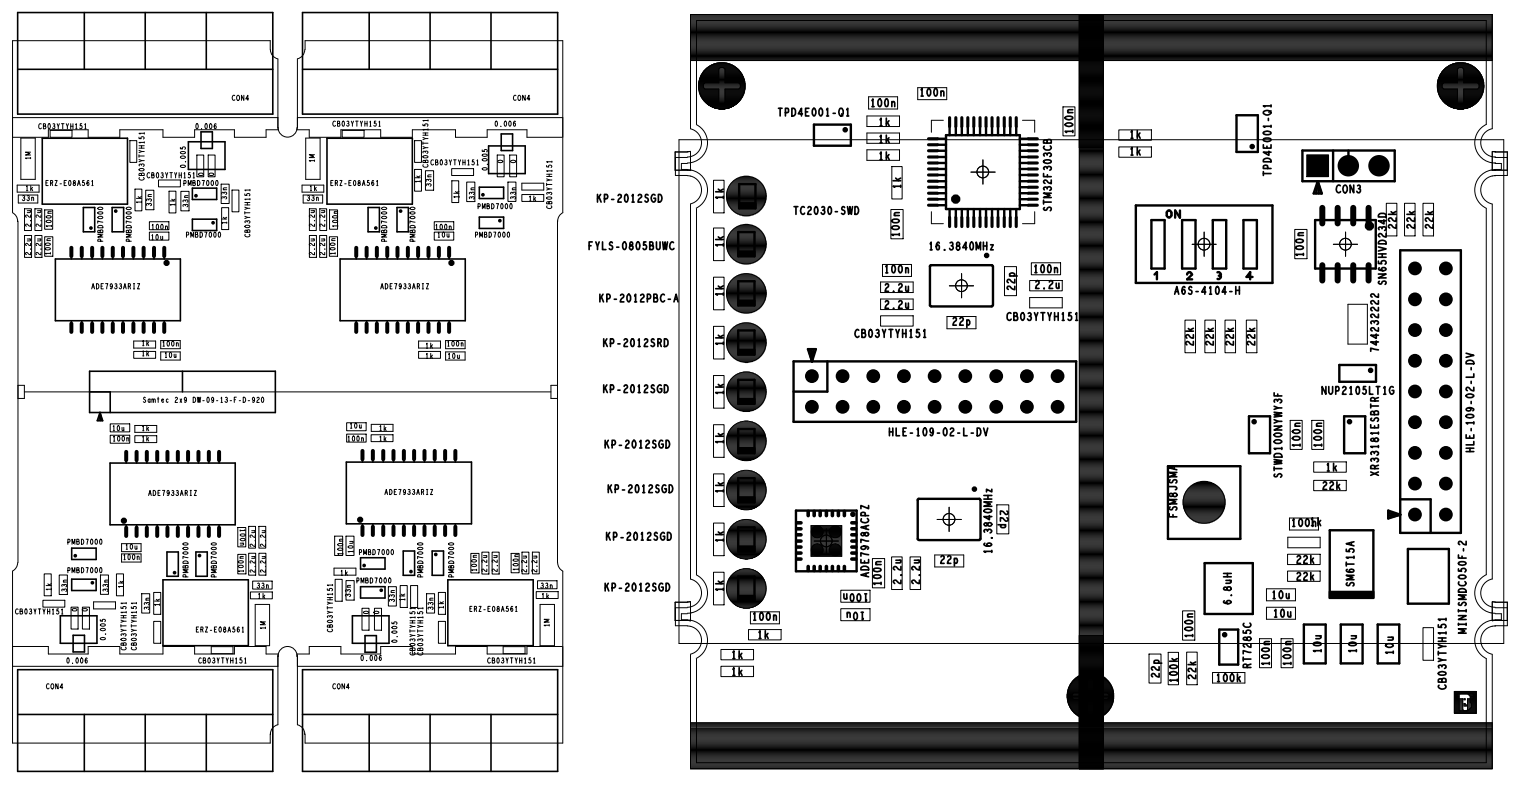
\includegraphics[height=0.9\textheight]{figures/4_4_1_CRPM3_PCB.png}
    \caption{CR-PM3A �s CR-PM3C be�ltet�si rajzai}
\end{figure}
\end{landscape}

\begin{figure}[!h]
\centering
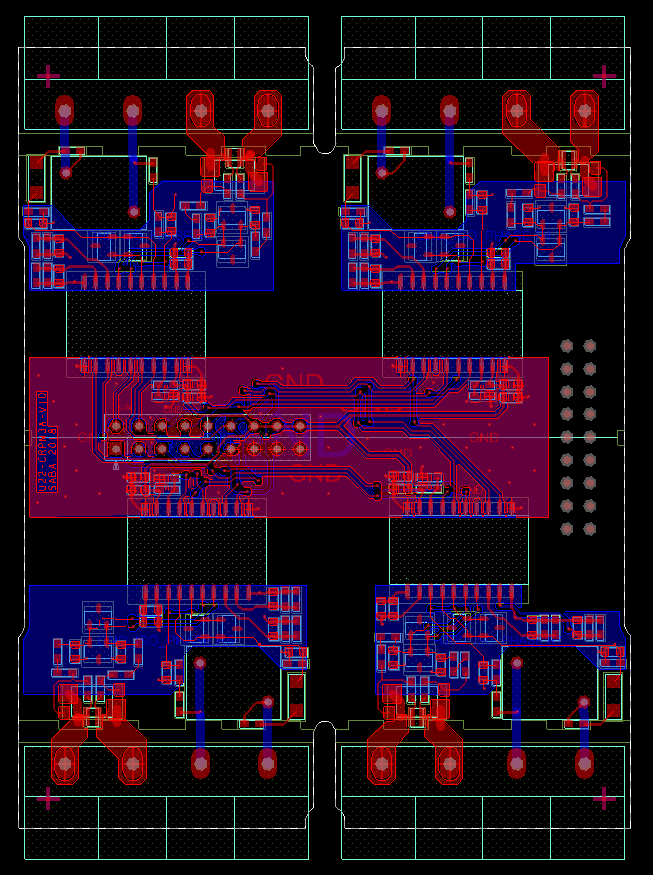
\includegraphics[width=150mm, keepaspectratio]{figures/CRPM3_A_EGESZ.PNG}
\caption{CR-PM3A NY�K terv�nek fel�ln�zeti k�pe}
\end{figure}

\begin{landscape}
\begin{figure}[!h]
   \centering
    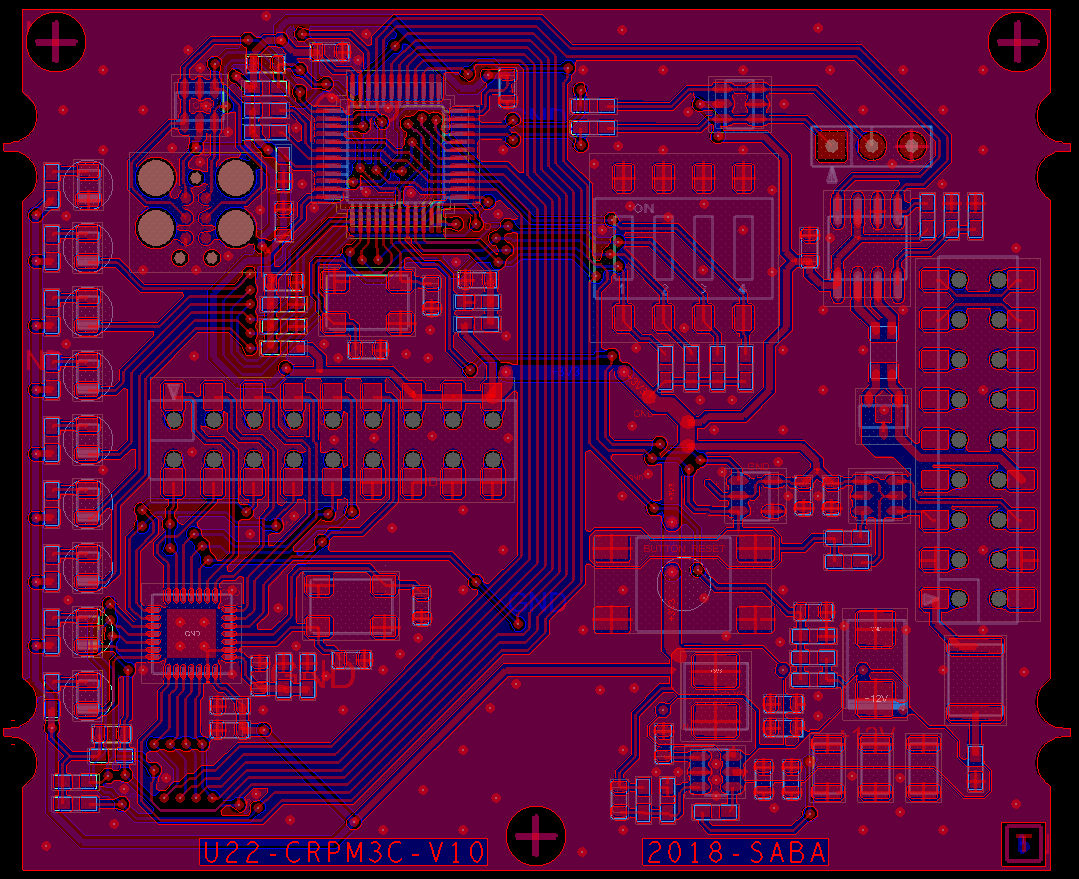
\includegraphics[height=0.9\textheight]{figures/CRPM3_C_EGESZ.PNG}
    \caption{CR-PM3C NY�K terv�nek fel�ln�zeti k�pe}
\end{figure}
\end{landscape}

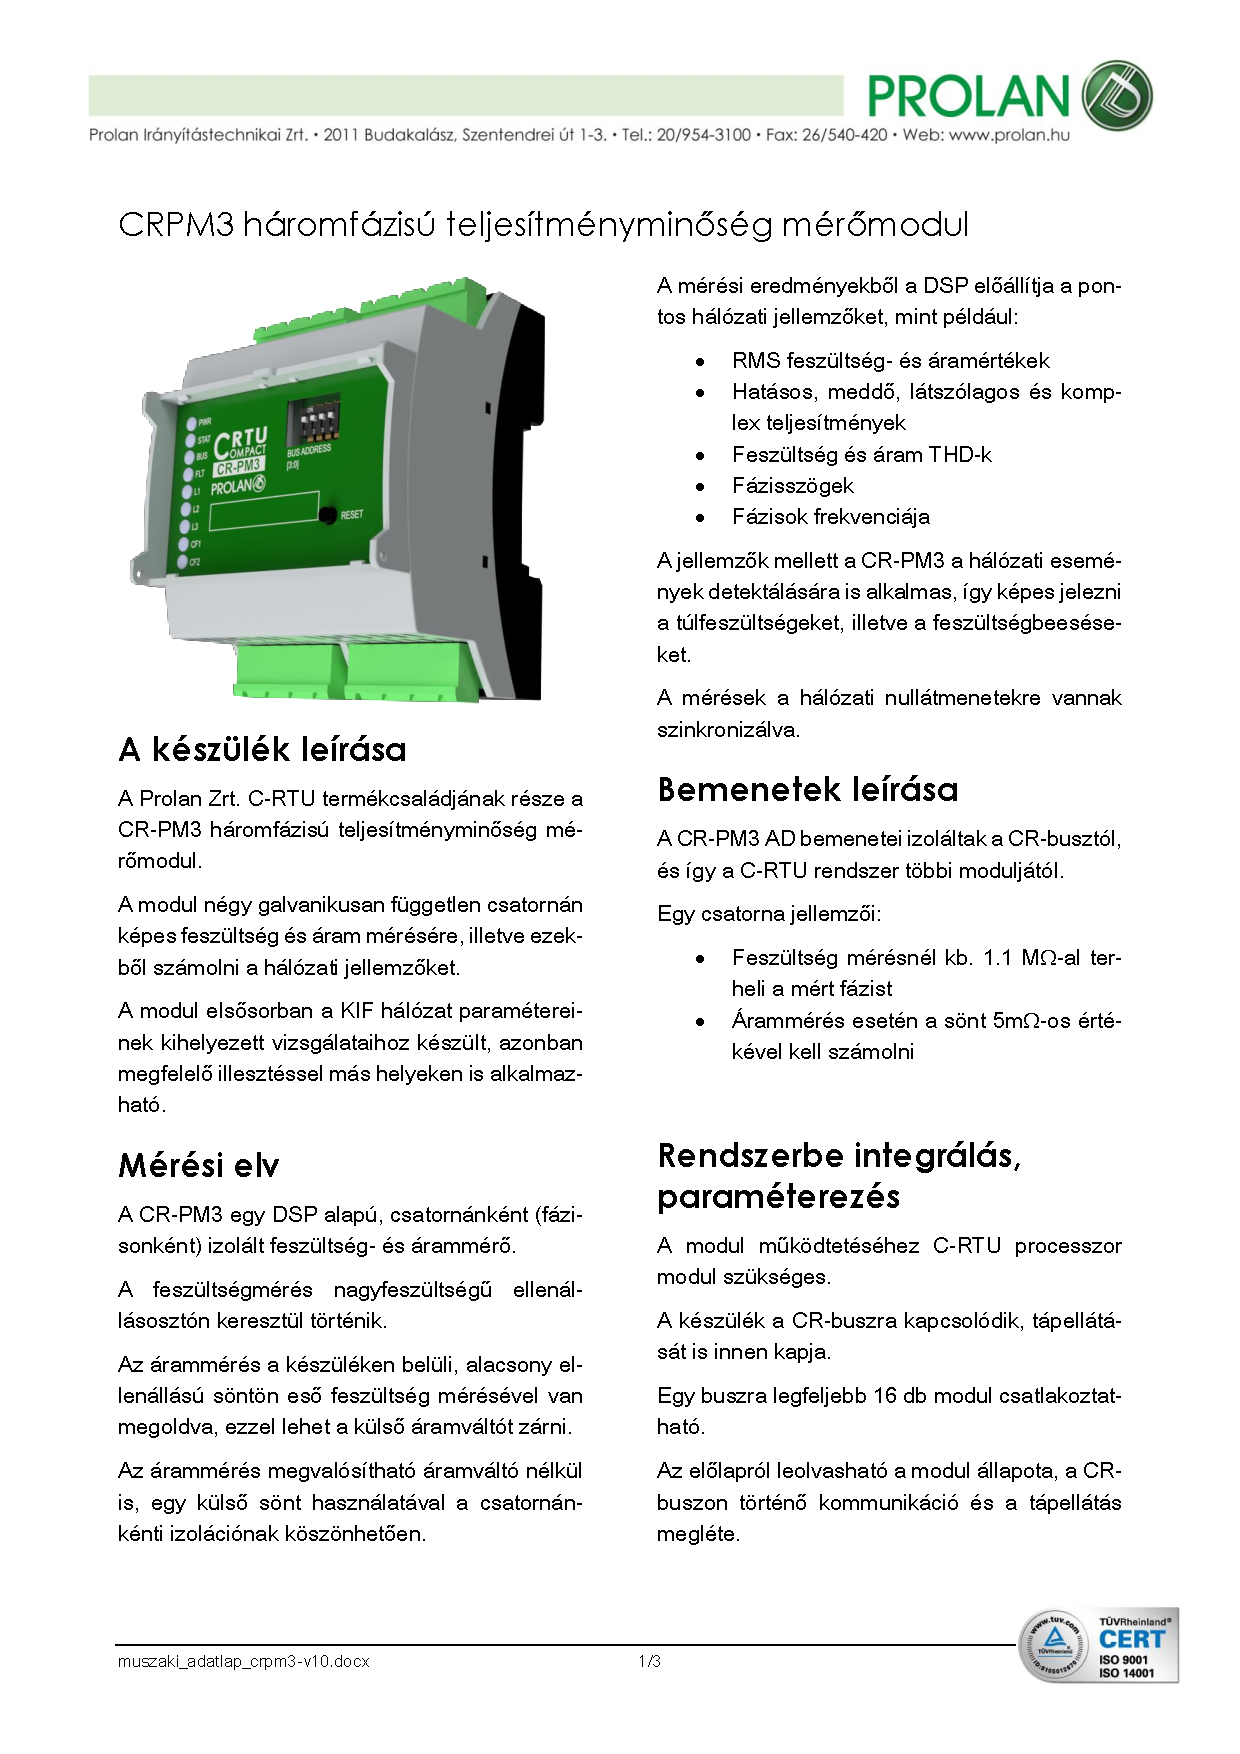
\includepdf[pages=-]{figures/Muszaki_adatlap_CRPM3-V10.pdf}